\documentclass{beamer}
  \usepackage{D:/cours/INGESUP/package/model_slide}    
  
  \begin{document}
  
  \title{Listes d'exercices Module04  }
  \subtitle{Statistiques}
  \maketitle

  \begin{frame} % premier transparent
  \frametitle{Statistiques}
  \begin{exercice}[1]
   Soit un véhicule qui avance à 10km/h sur une distance de 20km puis augmente sa vitesse et avance à 120km/h sur une distance de 200km. Calculer la moyenne des vitesses sur l'ensemble du parcours. \\
   $t_1 = \frac{20}{10} = 2h$ et $t_2=\frac{200}{120} = \frac{5}{3} h$ 
   \\ et donc $\bar{v} = \frac{220}{2 + \frac{5}{3}} = \frac{220}{\frac{11}{3}} = 220 \times \frac{3}{11} = 60 km/h$. cette moyenne est appelée moyenne harmonique.
  \end{exercice}

\end{frame}

\begin{frame} % deuxième transparent
  \frametitle{Statistiques}
  \begin{exercice}[2.1]
    Moyenne
    \begin{figure}[!h]
      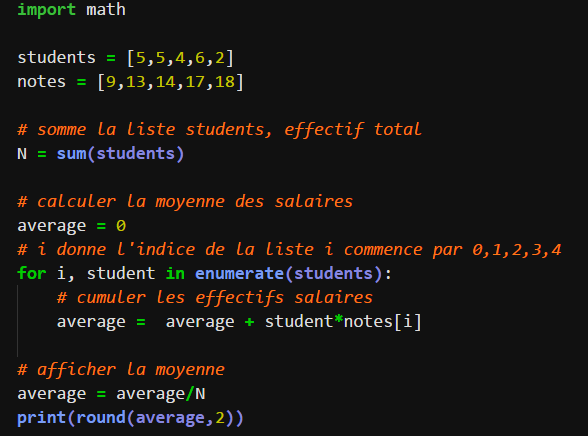
\includegraphics[width=8cm]{../Images/stat_exo21_corr}
  \end{figure} 
  \end{exercice}

\end{frame}

\begin{frame} % deuxième transparent
  \frametitle{Statistiques}
  \begin{exercice}[2.1]
    Variance et écart type
    \begin{figure}[!h]
      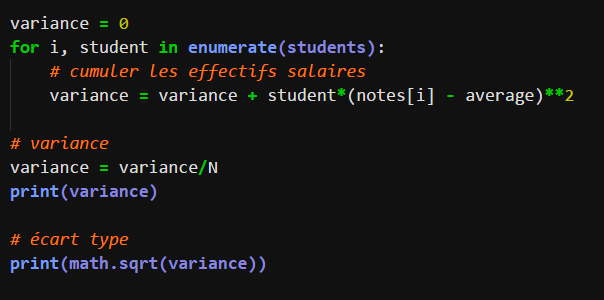
\includegraphics[width=4cm]{../Images/stat_exo22_corr}
  \end{figure} 
  \end{exercice}

\end{frame}

\begin{frame} % deuxième transparent
  \frametitle{Statistiques}
  \begin{exercice}[2.2]
   Mediane Challenge Python
    \begin{figure}[!h]
      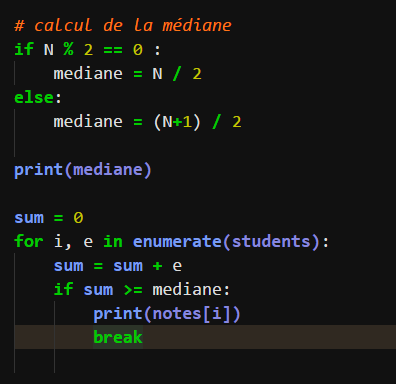
\includegraphics[width=4cm]{../Images/stat_exo23_corr}
  \end{figure} 
  \end{exercice}

\end{frame}

\begin{frame} % deuxième transparent
  \frametitle{Statistiques}
  \begin{exercice}[3.1]
    Droite de régression et nuage de points
    \begin{figure}[!h]
      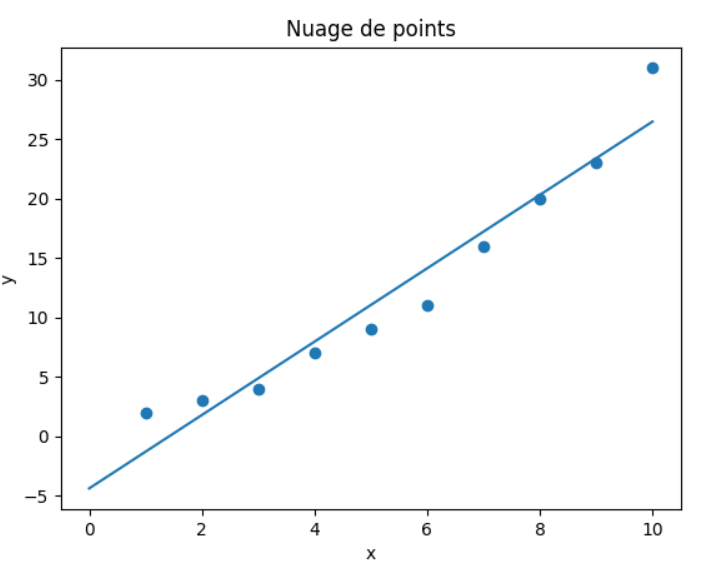
\includegraphics[width=4cm]{../Images/stat_exo33_corr}
  \end{figure}
  \end{exercice}

\end{frame}

\begin{frame} % deuxième transparent
  \frametitle{Statistiques}
  \begin{exercice}[3.2]
      Scripts Python
      \begin{figure}[!h]
        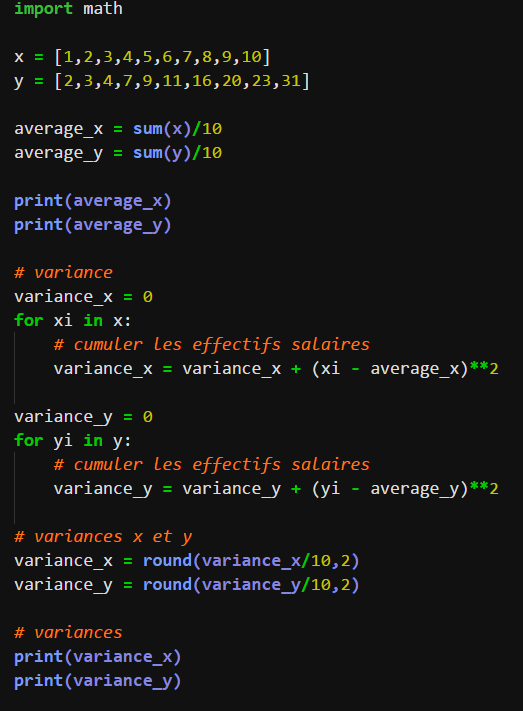
\includegraphics[width=4cm]{../Images/stat_exo32_corr}
    \end{figure}
  \end{exercice}

\end{frame}


\begin{frame} % dernière transparent
 Fin des exercices sur le probabilité, merci de les avoir suivis.
\end{frame}
  
\end{document}